\section{TP3}
\label{chap:Mini Projet}

\subsection{Commencement}

\noindent \textbf{Durée : 3h}: \\
\noindent Au cours de ce TP, vous allez devoir attaquer la machine \textbf{TP3-CTF}. Le but du TP est de récupérer un flag et d'obtenir une élévation de privilège sur la machine adverse.\\

\noindent Rendez vous sur le FTP de l'IUT à l'adresse \textbf{ftp://192.168.33.54} et téléchargez le CTF au format OVA \textbf{TP3-CTF.ova}. Installez-le sur votre machine avec Virtualbox. Si ce n'est pas déjà fait, téléchargez un iso de Kali linux sur le ftp de l'IUT ou demandez une image aux encadrants.

\subsubsection{Configuration réseau de Virtualbox}

Pour effectuer ce TP, vous allez configurer un réseau NAT sous Virtualbox. Vous allez tout d'abord créer un réseau NAT pour faire communiquer votre Kali Linux et la machine qui hébergera le CTF. Pour ce faire, allez dans \textbf{Fichier/Paramètres/Réseau}:

\begin{figure}[htp!]
  \centering
  \setlength\figureheight{7cm}
  \setlength\figurewidth{9cm}
  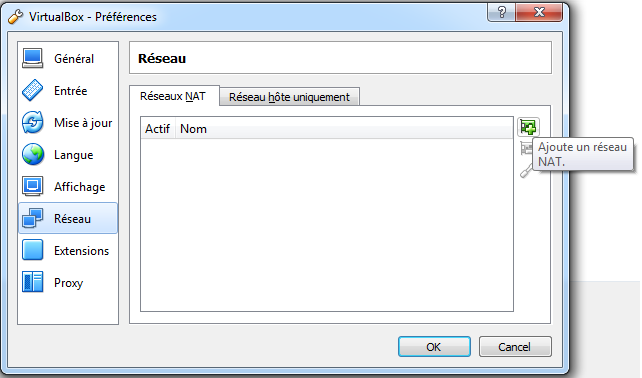
\includegraphics[width=0.5\textwidth]{oui/TP3/imageCTF.png}
  \caption{Création du réseau NAT}
  \label{fig:courbe-tikz}
\end{figure}

Appuyez sur le "+" pour créer votre réseau. Par défaut, ce réseau dispose d'un serveur DHCP avec une adresse réseau de \textbf{10.0.2.0/24} :
%\newpage
\begin{figure}[htp!]
  \centering
  \setlength\figureheight{7cm}
  \setlength\figurewidth{9cm}
  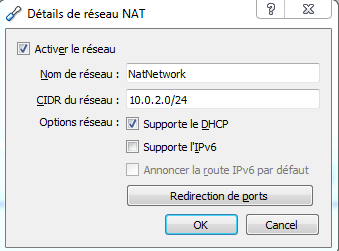
\includegraphics[width=0.5\textwidth]{oui/TP3/imageCTF2.png}
  \caption{Paramètres réseau NAT}
  \label{fig:courbe-tikz}
\end{figure}

Vous pouvez laisser tout par défaut.

\subsubsection{Ajout d'une machine au réseau}

Pour ajouter votre VM au réseau NAT, selectionnez votre machine, cliquez sur configuration. Allez ensuite dans la catégorie réseau et sélectionnez réseau NAT:

\begin{figure}[htp!]
  \centering
  \setlength\figureheight{7cm}
  \setlength\figurewidth{9cm}
  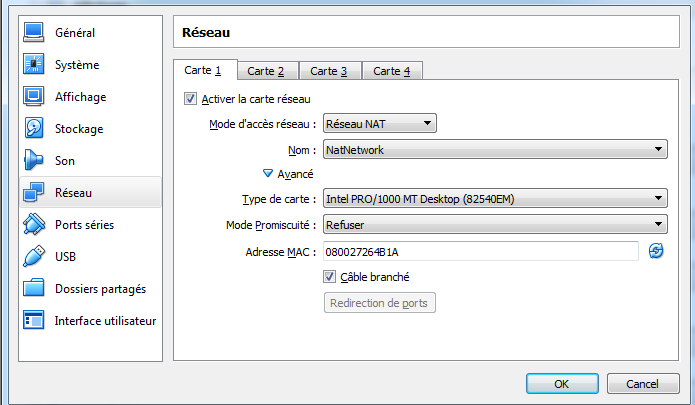
\includegraphics[width=0.7\textwidth]{oui/TP3/imageCTF3.png}
  \caption{Aujout d'une machine au réseau NAT}
  \label{fig:courbe-tikz}
\end{figure}

Effectuez cette opération pour votre Kali linux ainsi que pour la machine TP3-CTF.